\section{Wrappers -- traditional Specification}

The figure needs some beautification

\begin{figure}[htb]
\begin{tabular}{llll}
\begin{lstlisting}
class Wrapper(nd,hgt){

  fld node=nd;
  fld height=hgt;

  func setPropety(i,prp)
  // PRE: i
  // POST:
  //     i>this.height -> modifies nothing
  //     &&
  //     i<=this.height -->
  //           modifies = { this.node.parent^i.property }
  //          &&
  //          this.node,parent^i.property == prp
  {
    if (i>height){ 
       return 
    } 
    else  
    {  nd=node;  
       while (i>0){
          nd=nd.getParent();
          i--;    };
        nd.setProperty(prp); }
  }    
  func getChild(i)
  
  { 
    Wrapper(node.getChild(i),
                    height+1); 
 }                           
}
\end{lstlisting}
\end{minipage}
\end{tabular}
 \vspace*{-7mm}
\caption{\prg{Node}  and \prg{Wrapper} }
\label{fig:DOM}
\end{figure}

In Figure \ref{fig:WrapperUse} we show an example of the use of  \prg{Wrapper} objects to attenuate the use of \prg{Node}s\footnote{SD: Is that a good sentence?}  The function \prg{usingWrappers} takes as parameter an object of unknown provenance, here called \prg{unknwn}. On lines 2-7 it creates a tree, consisting of nodes \prg{n1}, \prg{n2}, ... \prg{n6}, depicted as blue circles on the   right-hand-side of the Figure. On line 8 it creates a wrapper of \prg{n5} with height \prg{1}. This means that the wrapper \prg{w} may be used to modify \prg{n3}, \prg{n5} and \prg{n6} (\ie the objects in the green triangle), while it cannot be used to modify \prg{n1}, \prg{n2}, and \prg{4} (\ie the objects within the blue triangle). 
On line 8 we call   function \prg{untrusted} on the \prg{unknown} object, passing \prg{w} as   argument. 

\begin{figure}[htb]
\begin{tabular}{llll}
\ \ &
\begin{minipage}{0.35\textwidth}
\begin{lstlisting}
func usingWrappers(unknwn){
   n1=Node(null,"fixed"); 
   n2=Node(n1,"robust"); 
   n3=Node(n2,"volatile"); 
   n4=Node(n2,"const");
   n5=Node(n3,"variable");
   n6=Node(n3,"ethereal");
   w=Wrapper(n5,1);
   
   unknwn.untrusted(w);
   
   assert n2.property=="robust" 
   ...
}
\end{lstlisting}
\end{minipage}
& & 
\begin{minipage}{0.75\textwidth}
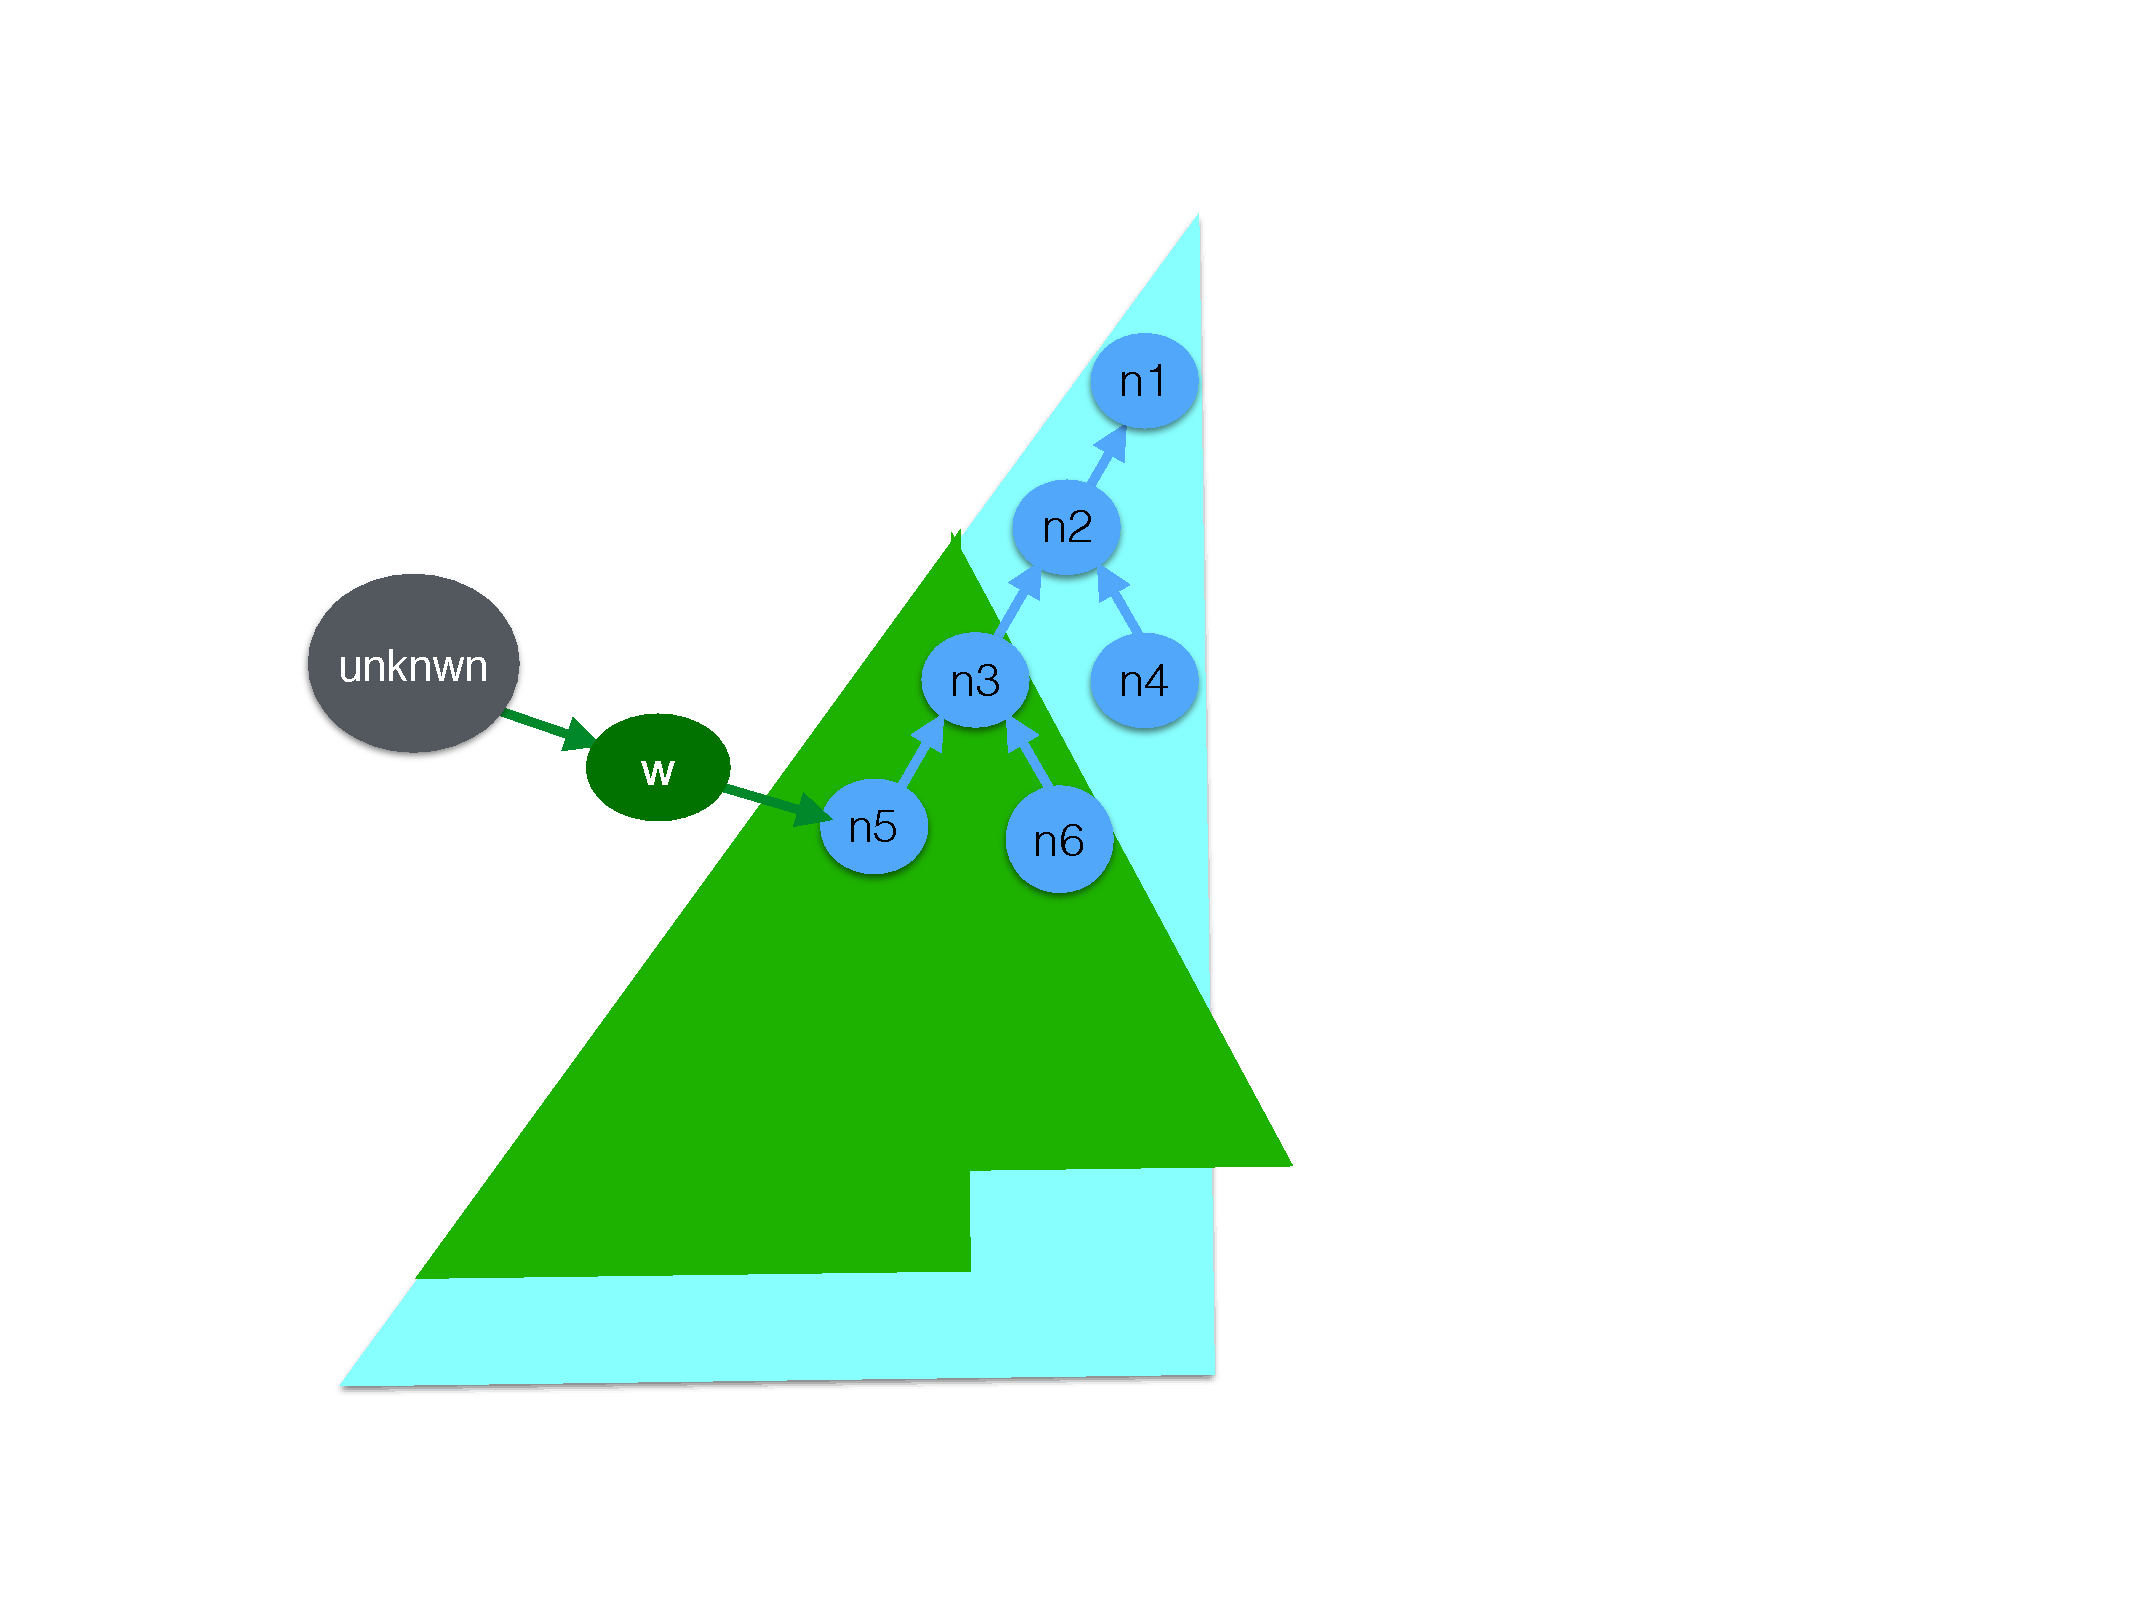
\includegraphics[width=\linewidth, trim=145  320 60 105,clip]{diagrams/DOM.pdf}
% x y z w
% y seems to eat up the bollom
% y=320 is good
% x eats space from left, if you increase it the diagram decreases from left
% w eats space from top, if you increase it the diagram decreases from top
% w=100 is good
%\includegraphics[page=3, width=\linewidth, trim=150  270 40 150, clip]{diagrams/snmalloc.pdf}\sdcomment{I think we need to change the diagram so that it says small slab.}
\strut \\
\strut \\

\end{minipage}
\end{tabular}
 \vspace*{-2.5mm}
\caption{\prg{Wrapper}s protecting \prg{Node}s }
\label{fig:WrapperUse}
\end{figure}

However, even though we know nothing about \prg{unknown} or \prg{untrusted}, and even though the call gives to \prg{unknown}  access to \prg{w}, which in turn has transitively access to all  \prg{Node}-s in the tree, 
we know that the call to the \prg{untrusted} function is guaranteed not to affect the   \prg{property} fields of the nodes \prg{n1}, \prg{n2}, and \prg{n4}. 
Thus, the assertion on line 10 is guaranteed to succeed. 
The question is how do we specify \prg{Wrapper}, so as to be able to prove this assertion.

We give a  specification of the class \prg{Wrapper}  in the appendix in the traditional specification style \cite{Leavens-etal07}.
 